\documentclass[a4paper,12pt]{article}
\usepackage{amsmath} \usepackage{amsthm}
\usepackage[croatian]{babel}
\usepackage{graphicx}
\usepackage{amssymb} \usepackage{fancybox}
\usepackage{latexsym}
\usepackage{enumerate}
\usepackage{subcaption}
\addtolength{\hoffset}{-1cm} \addtolength{\textwidth}{2cm}
\addtolength{\topmargin}{-2.5cm} \addtolength{\textheight}{3cm}

\newtheoremstyle{zad}% name
  {0.3cm}%      Space above
  {10pt}%      Space below
  {}%         Body font
  {}%         Indent amount (empty = no indent, \parindent = para indent)
  {\bf}% Thm head font
  {.}%        Punctuation after thm head
  {\newline}%     Space after thm head: " " = normal interword space;
        %       \newline = linebreak
  {}%         Thm head spec (can be left empty, meaning `normal')

\theoremstyle{zad}
\newtheorem{zadatak}{Zadatak}

\begin{document}
%\thispagestyle{empty}
\begin{center}
\shadowbox{\Large Ulančani torusi}\\[2pt]
\end{center}
Torus je ploha koja ima implicitnu jednad\v{z}bu
$$\big(x^2+y^2+z^2+R^2-r^2\big)^2-4R^2\big(x^2+y^2\big)=0.$$
Za razli\v{c}ite odabire konstanti $R$ i $r$ dobivamo druk\v{c}ije toruse.\\[5pt]
Dvostruki torus nastaje lijepljenjem dva torusa. Proces lijepljenja odgovara produktu
implicitnih jednad\v{z}bi torusa umanjenom za neku konstantu. Konkretnije, implicitna
jednad\v{z}ba dvostrukog torusa glasi
$$f_1(x,y,z)\cdot f_2(x,y,z)=c,$$
pri \v{c}emu je
\begin{align*}
f_1(x,y,z)&=\big((x+a)^2+y^2+z^2+R^2-r^2\big)^2-4R^2\big((x+a)^2+y^2\big)\\
f_2(x,y,z)&=\big((x+b)^2+y^2+z^2+R^2-r^2\big)^2-4R^2\big((x+b)^2+y^2\big)
\end{align*}
za neke odabrane konstante $a,b,c,r,R$.\\[5pt]
Trostruki torus nastaje lijepljenjem tri torusa. Mo\v{z}emo ga vizualizirati preko
implicitne jednad\v{z}be
$$g_1(x,y,z)\cdot g_2(x,y,z)\cdot g_3(x,y,z)=c,$$
pri \v{c}emu je
\begin{align*}
g_1(x,y,z)&=\big((x+a)^2+y^2+z^2+R^2-r^2\big)^2-4R^2\big((x+a)^2+y^2\big)\\
g_2(x,y,z)&=\big((x+b_1)^2+(y+b_2)^2+z^2+R^2-r^2\big)^2-4R^2\big((x+b_1)^2+(y+b_2)^2\big)\\
g_3(x,y,z)&=\big((x+c_1)^2+(y+c_2)^2+z^2+R^2-r^2\big)^2-4R^2\big((x+c_1)^2+(y+c_2)^2\big)
\end{align*}
i vrijedi $b_1=a\cos{\frac{2}{3}\pi}$, $b_2=a\sin{\frac{2}{3}\pi}$, $c_1=a\cos{\frac{4}{3}\pi}$,
$c_2=a\sin{\frac{4}{3}\pi}$ za neke odabrane\vspace*{2pt} konstante $a,c,r,R$.\par
\begin{figure}[!h]
\centering
\subcaptionbox{dvostruki torus}{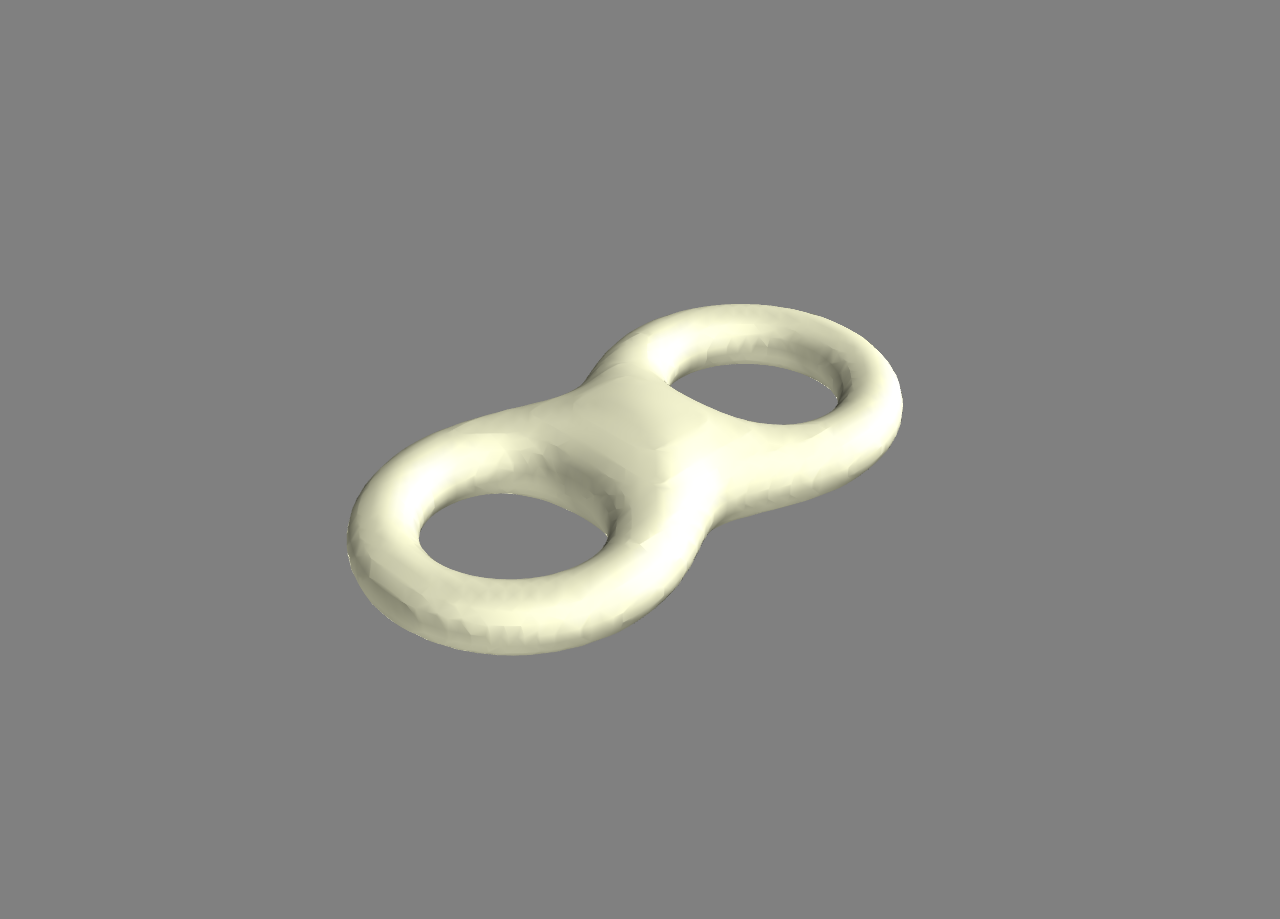
\includegraphics[scale=0.12]{dvostrukiTorus.png}}\hspace*{0.5cm}
\subcaptionbox{trostruki torus}{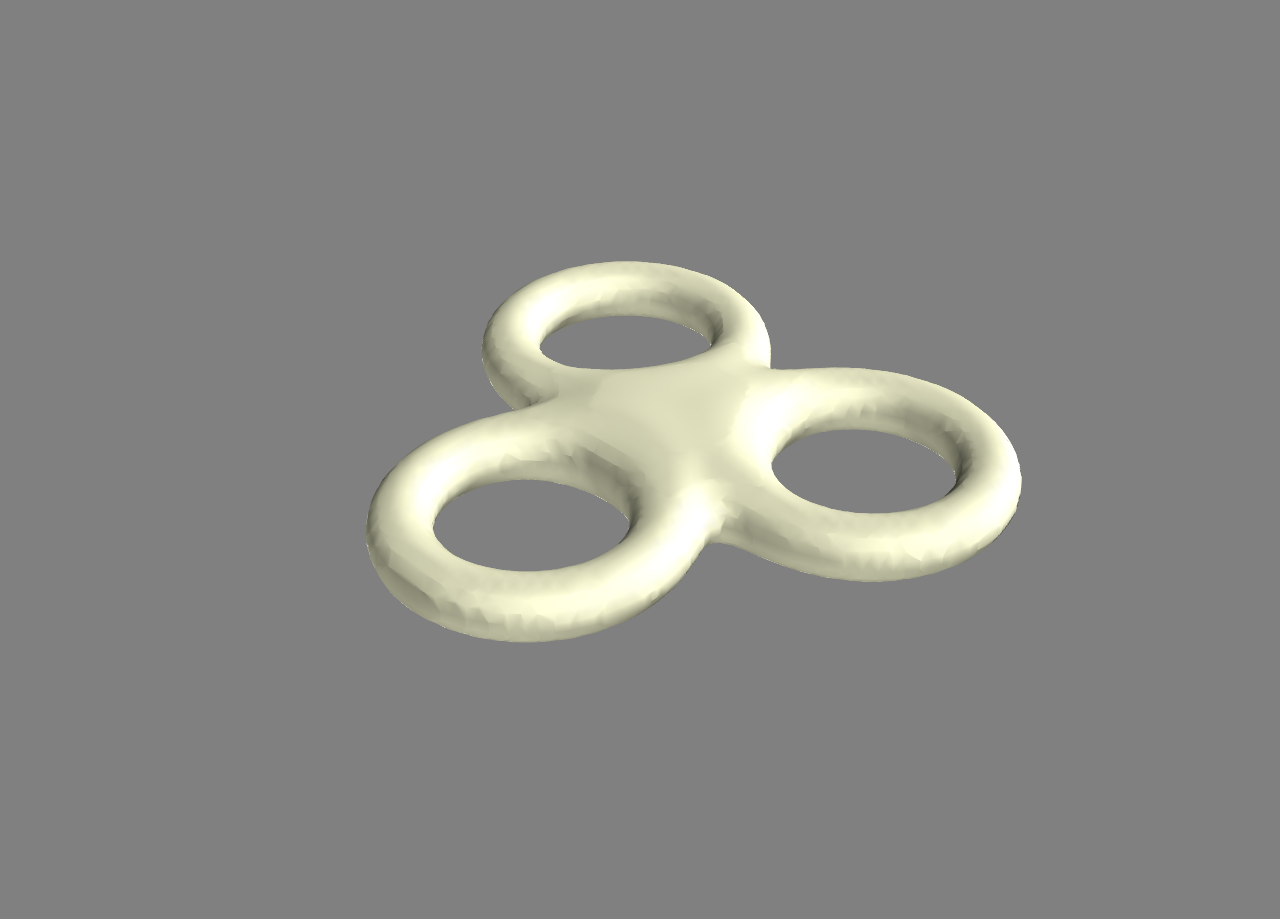
\includegraphics[scale=0.12]{trostrukiTorus.png}}\hspace*{0.5cm}
\caption{Dvostruki i trostruki torus}
\end{figure}
\noindent Pomo\'cu dvostrukog i trostrukog torusa možemo napraviti 3D model koji se sastoji od dva tro\-stru\-ka torusa 
i tri dvostruka torusa koji su raspore\dj eni na na\v{c}in kako je prikazano na slici \ref{model}.

\newpage

\begin{figure}
\centering
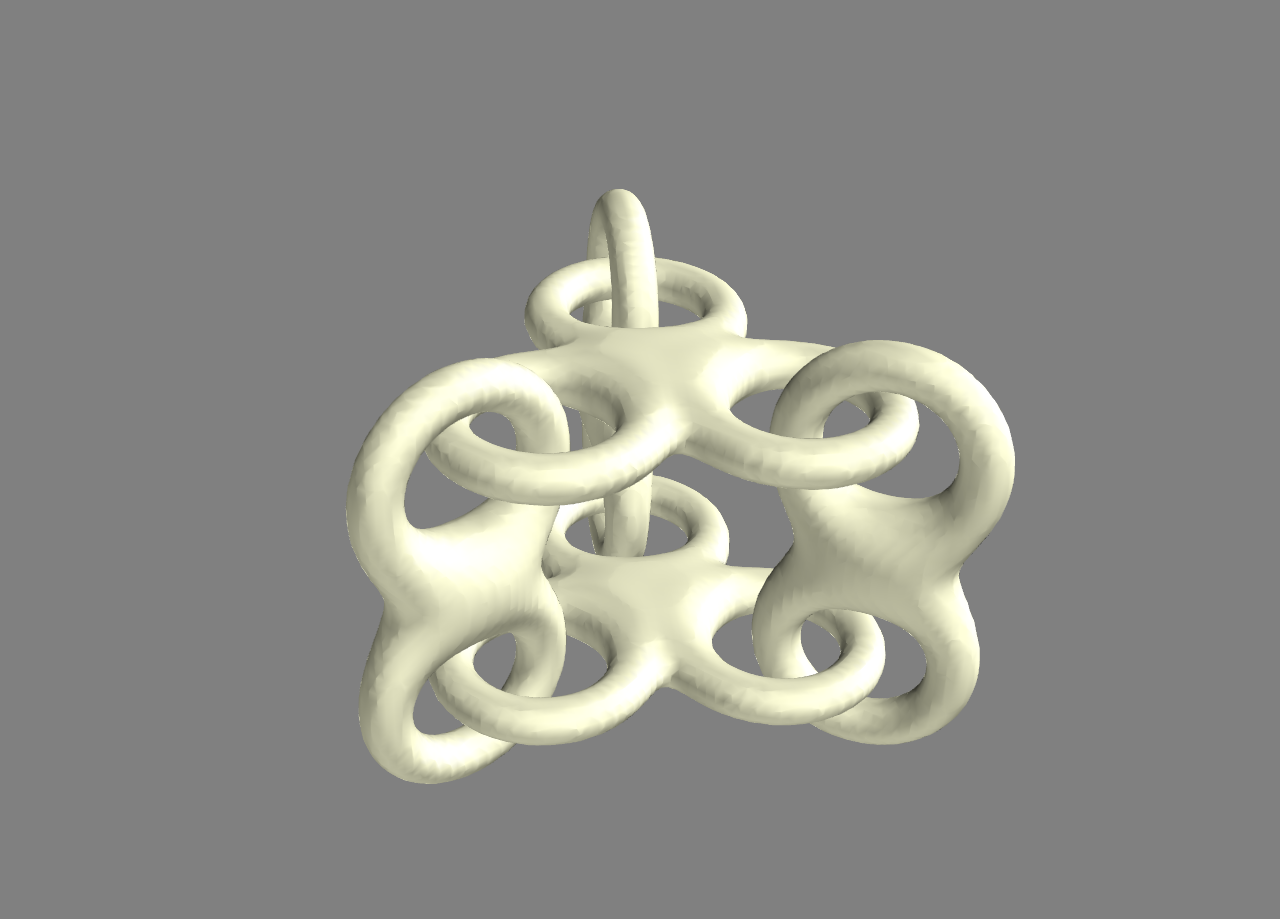
\includegraphics[scale=0.12]{torusi1.png}
\caption{Ulančani torusi}\label{model}
\end{figure}

\noindent Za dovođenje dvostrukih i trostrukih torusa u željeni položaj treba na njihove standardne implicitne jednadžbe
primijeniti određene transformacije: translacije i rotacije oko koordinatnih osi.\\[3pt]
Translacija za vektor $(x_0,y_0,z_0)$ preslikava to\v{c}ku $(x,y,z)$ u to\v{c}ku
$(x+x_0,y+y_0,z+z_0)$, tj. matemati\v{c}ki zapisano
$$(x,y,z)\mapsto(x+x_0,y+y_0,z+z_0).$$
Rotacija $R_{x,\phi}$ oko osi $x$ za kut $\phi$, rotacija $R_{y,\phi}$ oko osi $y$ za kut $\phi$, rotacija $R_{z,\phi}$ oko osi $z$ za kut $\phi$ imaju redom
matri\v{c}ne prikaze
$$
R_{x,\phi}=\begin{bmatrix}1&0&0\\ 0&\cos{\phi}&-\sin{\phi}\\ 0&\sin{\phi}&\cos{\phi}\end{bmatrix},\
R_{y,\phi}=\begin{bmatrix}\cos{\phi}&0&\sin{\phi}\\ 0&1&0\\ -\sin{\phi}&0&\cos{\phi}\end{bmatrix},\
R_{z,\phi}=\begin{bmatrix}\cos{\phi}&-\sin{\phi}&0\\ \sin{\phi}&\cos{\phi}&0\\ 0&0&1\end{bmatrix}.
$$
Na primjer, rotacija oko osi $x$ za kut $\phi$ preslikava to\v{c}ku $(x,y,z)$ u to\v{c}ku
$$
\begin{bmatrix}1&0&0\\ 0&\cos{\phi}&-\sin{\phi}\\ 0&\sin{\phi}&\cos{\phi}\end{bmatrix}\begin{bmatrix}x\\ y\\ z\end{bmatrix}=
\begin{bmatrix}x\\ y\cos{\phi}-z\sin{\phi}\\ y\sin{\phi}+z\cos{\phi}\end{bmatrix}
$$
odnosno
$$(x,y,z)\mapsto (x,\,y\cos{\phi}-z\sin{\phi},\,y\sin{\phi}+z\cos{\phi}).$$
\textbf{Va\v{z}na napomena.} Gornji matri\v{c}ni prikazi rotacija su prikazi pozitivnih rotacija u desnom koordinatnom sustavu.
\v{S}to se ti\v{c}e stavljanja minus predznaka kod sinus \v{c}lana, ukoliko ne brinemo previ\v{s}e o tome kod kojeg \'cemo ga \v{c}lana staviti, onda moramo paziti na jednu stvar. Ukoliko, na primjer, nekim slu\v{c}ajem rotacijom objekta oko $x$-osi za $30^{\circ}$ nismo dobili \v{z}eljeni polo\v{z}aj objekta, a mi smo gotovo pa sigurni da mora biti rotacija za taj kut, onda je mo\v{z}da samo problem da smo vjerojatno trebali rotirati za $-30^{\circ}$. Upravo izbor sinus \v{c}lana kod kojeg \'cemo staviti minus predznak u matrici rotacije bitno utje\v{c}e na pozitivne i negativne kutove. Zapravo to jako ovisi i o tome da li imamo lijevi ili desni koordinatni sustav (pazite, neki 3D programi koriste desni, a neki lijevi koordinatni sustav). No, jednostavno re\v{c}eno, ako niste dobili o\v{c}ekivani efekt rotacijom za neki kut $\phi$, probajte rotirati za kut $-\phi$.  
 
\end{document}
